% Source: graduate-coursework/Prior_Semesters/Fa24/EMCH367/assignments/hw1/hw1.tex

\documentclass[border=4pt]{standalone}
\usepackage{amsmath}
\usepackage{amssymb}
\usepackage{graphicx}
\usepackage{tikz}
\usepackage{xcolor}

\begin{document}
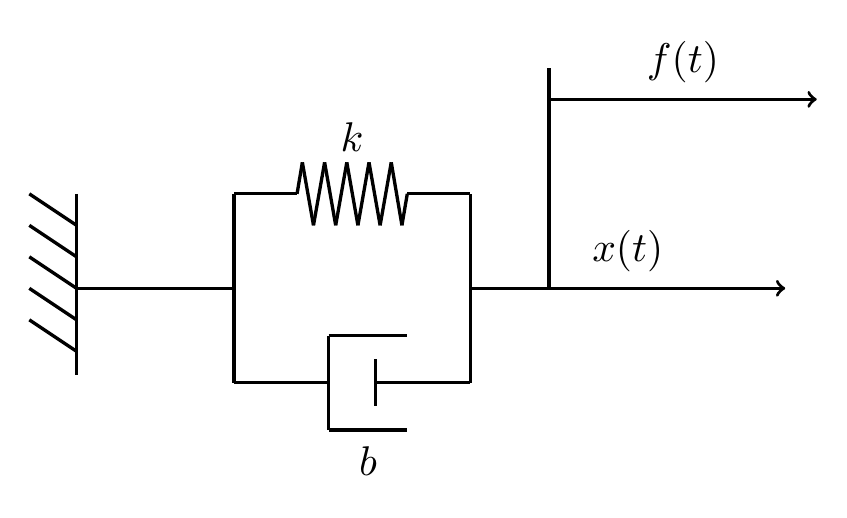
\begin{tikzpicture}[scale=0.4]
		% Multiple line segments with coordinates adjusted and line width increased
		\draw[line width=1.2pt] (0,6) -- (1.5,5);  % From (0,6) to (1.5,5)
		\draw[line width=1.2pt] (0,5) -- (1.5,4);  % From (0,5) to (1.5,4)
		\draw[line width=1.2pt] (0,4) -- (1.5,3);  % From (0,4) to (1.5,3)
		\draw[line width=1.2pt] (0,3) -- (1.5,2);  % From (0,3) to (1.5,2)
		\draw[line width=1.2pt] (0,2) -- (1.5,1);  % From (0,2) to (1.5,1)
				
		% Vertical line with coordinates adjusted and line width increased
		\draw[line width=1.2pt] (1.5,6) -- (1.5,0.25);  % Vertical line from (1.5,6) to (1.5,0.25)
				
		% Horizontal line with coordinates adjusted and line width increased
		\draw[line width=1.2pt] (1.5,3) -- (6.5,3);  % Horizontal line from (1.5,3) to (6.5,3)
		\draw[line width=1.2pt] (6.5,6) -- (6.5,0);
				    
		% Horizontal lines and line width increased
		\draw[line width=1.2pt] (6.5,0) -- (9.5,0);
		\draw[line width=1.2pt] (6.5,6) -- (8.5,6);
				
		% Vertical line and line width increased
		\draw[line width=1.2pt] (9.5,-1.5) -- (9.5,1.5);
				
		% Additional horizontal lines at -1.5 and 1.5 y-coordinates and line width increased
		\draw[line width=1.2pt] (9.5,-1.5) -- (12,-1.5);
		\draw[line width=1.2pt] (9.5,1.5) -- (12,1.5);
				
		% Vertical line at x = 11, and horizontal through x = 11 and line width increased
		\draw[line width=1.2pt] (11,0.75) -- (11,-0.75);
		\draw[line width=1.2pt] (11,0) -- (14,0);
		\draw[line width=1.2pt] (14,0) -- (14, 6);
		\draw[line width=1.2pt] (14,6) -- (12, 6);
				
		% Initial shifts and settings
		\def\xShift{8.33}
		\def\yShift{6} % Shifting everything to start at y = 6 for the intersection
				    
		% Draw the spring with adjustments and line width increased
		\draw[line width=1.2pt] (8.5, 6) -- (8.669, 7.0);
		\draw[line width=1.2pt] (8.669, 7) -- (9.022, 5.0);
		\draw[line width=1.2pt] (9.022, 5) -- (9.375, 7.0);
		\draw[line width=1.2pt] (9.375, 7) -- (9.727, 5.0);
		\draw[line width=1.2pt] (9.727, 5) -- (10.08, 7);
		\draw[line width=1.2pt] (10.08, 7) -- (10.433, 5.0);
		\draw[line width=1.2pt] (10.433, 5) -- (10.785, 7);
		\draw[line width=1.2pt] (10.785, 7) -- (11.138, 5.0);
		\draw[line width=1.2pt] (11.138, 5) -- (11.491, 7);
		\draw[line width=1.2pt] (11.491, 7) -- (11.83, 5);
		\draw[line width=1.2pt] (11.83, 5) -- (12,6);
				    
		% Draw arrow for displacement x(t) with larger text
		\draw[->, line width=1.2pt] (14,3) -- (24,3) node[midway, above, scale=1.5] {$x(t)$};
				    
		% Draw force arrow f(t) with larger text
		\draw[->, line width=1.2pt] (16.5,9) -- (25,9) node[midway, above, scale=1.5] {$f(t)$};
				    
		% Label for k (spring constant) with larger text
		\node[scale=1.5] at (10.25,7.8) {$k$};
				    
		% Label for b (damper constant) with larger text
		\node[scale=1.5] at (10.75,-2.5) {$b$};
				
		% Additional lines and adjustments with increased line width
		\draw[line width=1.2pt] (14,3) -- (14,0);  % Downward line from the end of x(t) arrow
		\draw[line width=1.2pt] (16.5, 3) -- (16.5,10);
	\end{tikzpicture}
\end{document}
